\documentclass[tikz,border=2pt]{standalone}
\usepackage{amsmath,amssymb}
\usepackage{tikz}
\usetikzlibrary{matrix}

\begin{document}
% Assignment problem: 3 agents, 3 tasks, cost matrix; choose one entry per row and column
% with minimum total cost (rows 1,2,3 -> tasks 1,3,2, cost 4 + 7 + 1 = 12).
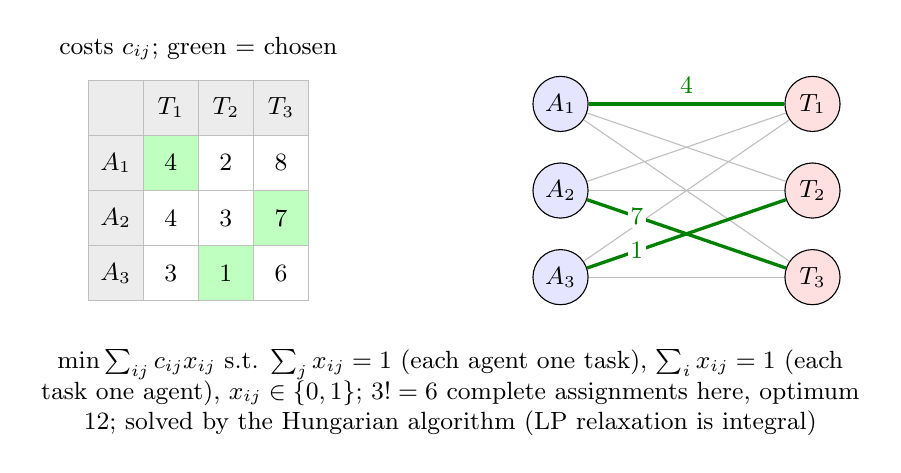
\begin{tikzpicture}[every node/.style={font=\small}, v/.style={draw, circle, fill=blue!10, minimum size=7mm, inner sep=0pt}, w/.style={draw, circle, fill=red!12, minimum size=7mm, inner sep=0pt}]
	\matrix (C) [matrix of math nodes, nodes={minimum size=7mm, anchor=center, draw=gray!50}, column sep=-\pgflinewidth, row sep=-\pgflinewidth] at (0,0) {
		|[fill=gray!15]| & |[fill=gray!15]| T_1 & |[fill=gray!15]| T_2 & |[fill=gray!15]| T_3 \\
		|[fill=gray!15]| A_1 & |[fill=green!25]| 4 & 2 & 8 \\
		|[fill=gray!15]| A_2 & 4 & 3 & |[fill=green!25]| 7 \\
		|[fill=gray!15]| A_3 & 3 & |[fill=green!25]| 1 & 6 \\
	};
	\node[anchor=south, font=\small] at (C.north) {costs $c_{ij}$; green = chosen};
	\begin{scope}[xshift=4.6cm]
		\foreach \i in {1,2,3} {\node[v] (a\i) at (0,{2.2-1.1*\i}) {$A_\i$};}
		\foreach \j in {1,2,3} {\node[w] (t\j) at (3.2,{2.2-1.1*\j}) {$T_\j$};}
		\foreach \i/\j in {1/2, 1/3, 2/1, 2/2, 3/1, 3/3} {\draw[gray!50] (a\i) -- (t\j);}
		\draw[green!50!black, very thick] (a1) -- (t1) node[midway, above, font=\small] {$4$};
		\draw[green!50!black, very thick] (a2) -- (t3) node[pos=0.25, font=\small, fill=white, inner sep=1pt] {$7$};
		\draw[green!50!black, very thick] (a3) -- (t2) node[pos=0.25, font=\small, fill=white, inner sep=1pt] {$1$};
	\end{scope}
	\node[anchor=north, align=flush center, text width=10.5cm] at (3.2,-1.9) {$\min\sum_{ij}c_{ij}x_{ij}$ s.t. $\sum_jx_{ij}=1$ (each agent one task), $\sum_ix_{ij}=1$ (each task one agent), $x_{ij}\in\{0,1\}$; $3!=6$ complete assignments here, optimum $12$; solved by the Hungarian algorithm (LP relaxation is integral)};
\end{tikzpicture}
\end{document}
